\section{Metodología}

Se consideró utilizar el modelo de desarrollo evolutivo o prototipo evolutivo ya que construye una serie de grandes versiones
sucesivas de un producto. Sin embargo, mientras que la aproximación incremental presupone que el conjunto completo de
requerimientos es conocido al comenzar, el modelo evolutivo. En este modelo, los requerimientos son cuidadosamente
examinados, y sólo esos que son bien comprendidos son seleccionados para el primer incremento. Los desarrolladores construyen
una implementación parcial del sistema que recibe sólo estos requerimientos.
Aplicaremos la metodología de la siguiente forma:\\

\begin{itemize}
	\item Planificación: especificaremos los requerimientos que se necesitan en cada uno de los módulos para su correcto
funcionamiento.

	\item Desarrollo: se realizará el módulo y las pruebas de funcionamiento antes de proseguir para la retroalimentación del cliente.
	
	\item Retroalimentación de parte del cliente: las pruebas serán realizadas por el cliente para poder tener la retroalimentación y
así exponer al sistema a una prueba en el entorno que será utilizado finalmente.
	
	\item Modificaciones: si se requieren se realizaran mejoras de acuerdo a los resultados obtenidos por el cliente, de no tener
alguna modificación se pasara a la siguiente fase hasta terminar el sistema.\\

\end{itemize}


\begin{figure}
	\centering
	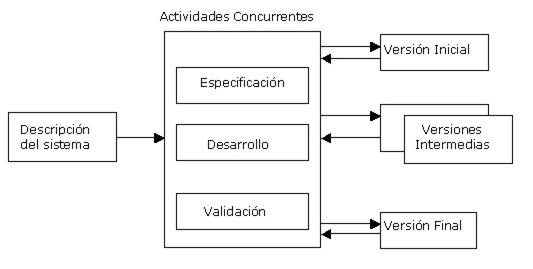
\includegraphics[scale=.7]{images/metodologia}
	\caption{Ciclo de vida de la metodología de prototipos.}
	\label{fig:metodologia}
\end{figure}


Los módulos del proyecto así como la documentación serán realizados en el siguiente orden:

\begin{itemize}
	\item Sensor y analizador
	
	\item Motor de interferencia
	
	\item Acciones de respuesta
	
	\item Registrador de eventos\\
\end{itemize}